\chapter{Technologies}
\section{WordPress}
\ac{wp} is one of the famous \ac{cms} that is powering almost 25\% of the websites globally. It is an Open Source project created, developed and maintained by the community. Hence, it can be downloaded, used, modified and distributed freely without any license fees.

The WordPress can be downloaded from their official website, \texttt{wordpress.org}. The current stable version of WordPress is 4.8, as at time of writing. Initially, it started as blogging system and became a full content management system with thousands of plugins, widgets and themes.

To run WordPress, the server should be equipped with \ac{php} version 7 or greater, MySQL database server version 5.6 or greater or MariaDB version 10.0 or greater, and \ac{http} support. As for web server, it is recommended to use either Apache or Nginx. They are reliable, have a lot of features, and works well with PHP and MySQL.

For Smart Home Lab website, WordPress will be ran using Nginx web server with PHP and MySQL. The Installation and configuration of them before installing WordPress will be discussed in the next chapter.

With WordPress, various website can be developed right from simple blogs to major websites comprising custom made plugins and widgets. This is one of the advantage of using WordPress is handling the flexibility and complexity while being easy to use.

Using WordPress enables the web developer to concentrate on the contents and structuring the websites, rather than developing the backend and frontend from scratch, which is time consuming and increased time to market.
Other than that, WordPress also provides multilingual pack consisting of 70 languages. This enable the website to developed in multiple languages, primarily in English and German languages. This not only changes the contents of the website as viewed by the web user, but also the administrator dashboard.

WordPress also provides excellent security for its users. Their security implementation consists of protection against Injection, Broken Authentication, \ac{xss}, Insecure Direct Object Reference, Security Misconfiguration etc. Their themes, plugins as well as hosting providers are tested and secured.

Using WordPress also make it easy for others to develop and continue the development of the website in the future, as everything can be managed in an easy web interface. And through this documentation, most of the essential information regarding the installation, configuration and contents development will be provided.

\section{PHP}
PHP stands for Hypertext Preprocessor. It is a general-purpose scripting language for generating dynamic web contents. It is commonly used for web development and can be embedded into HTML. The PHP scripts are executed on the server-side and the clients are unaware of the script and its execution. The result of the executed PHP will be sent to client in HTML format.

PHP scripts are processed by PHP parser or PHP interpreter. This parser will be installed in the web server such as Apache, IIC, lighttpd or Nginx as a \ac{cgi}. The PHP parser is open source software, which can be downloaded from their official website\footnote{http://php.net}.

PHP is not only limited to deliver web contents like HTML, but can be used to output text, images, PDFs and flash-videos. One of the PHP advantages is it supports and works well with various databases. For this website, the database called MySQL is used and will be discussed in the next section.

\section{MySQL}
MySQL is \ac{rdbms}. The Community Edition of MySQL is open source database system which can be downloaded from the official website\footnote{https://dev.mysql.com/downloads/}. MySQL uses \ac{sql} to query, filter, add, modify and delete data in the database. The data in the database will be arranged in table form. MySQL is used in majority of the websites and content management system such as WordPress.

\section{Nginx}
Nginx is a high-performance web server. It is also act as reverse proxy, IMAP/POP3 proxy server, load balancer and accelerator. It works with HTTP, \ac{tcp} as well as \ac{udp} based services. The main advantages of Nginx are its high performance, stability, rich feature set, simple configuration and low resource consumption.

The architecture of Nginx uses scalable event-drive asynchronous architecture. Not only it uses small amount of memory, but the memory usage is predictable under load. It success relies in the ability to handle thousands of requests at the same time. For this project, Nginx web server will be used, where it communicates with PHP parser to run WordPress and MySQL database.

\section{Microsoft Surface Hub}
Even though, the website designed for this thesis encompasses all range of devices from desktop to mobile devices, the main focus has been the Microsoft Surface Hub (see Figure~\ref{fig:surface-hub}).

\begin{figure}[ht]
\caption{Microsoft Surface Hub}
\label{fig:surface-hub}
\centering
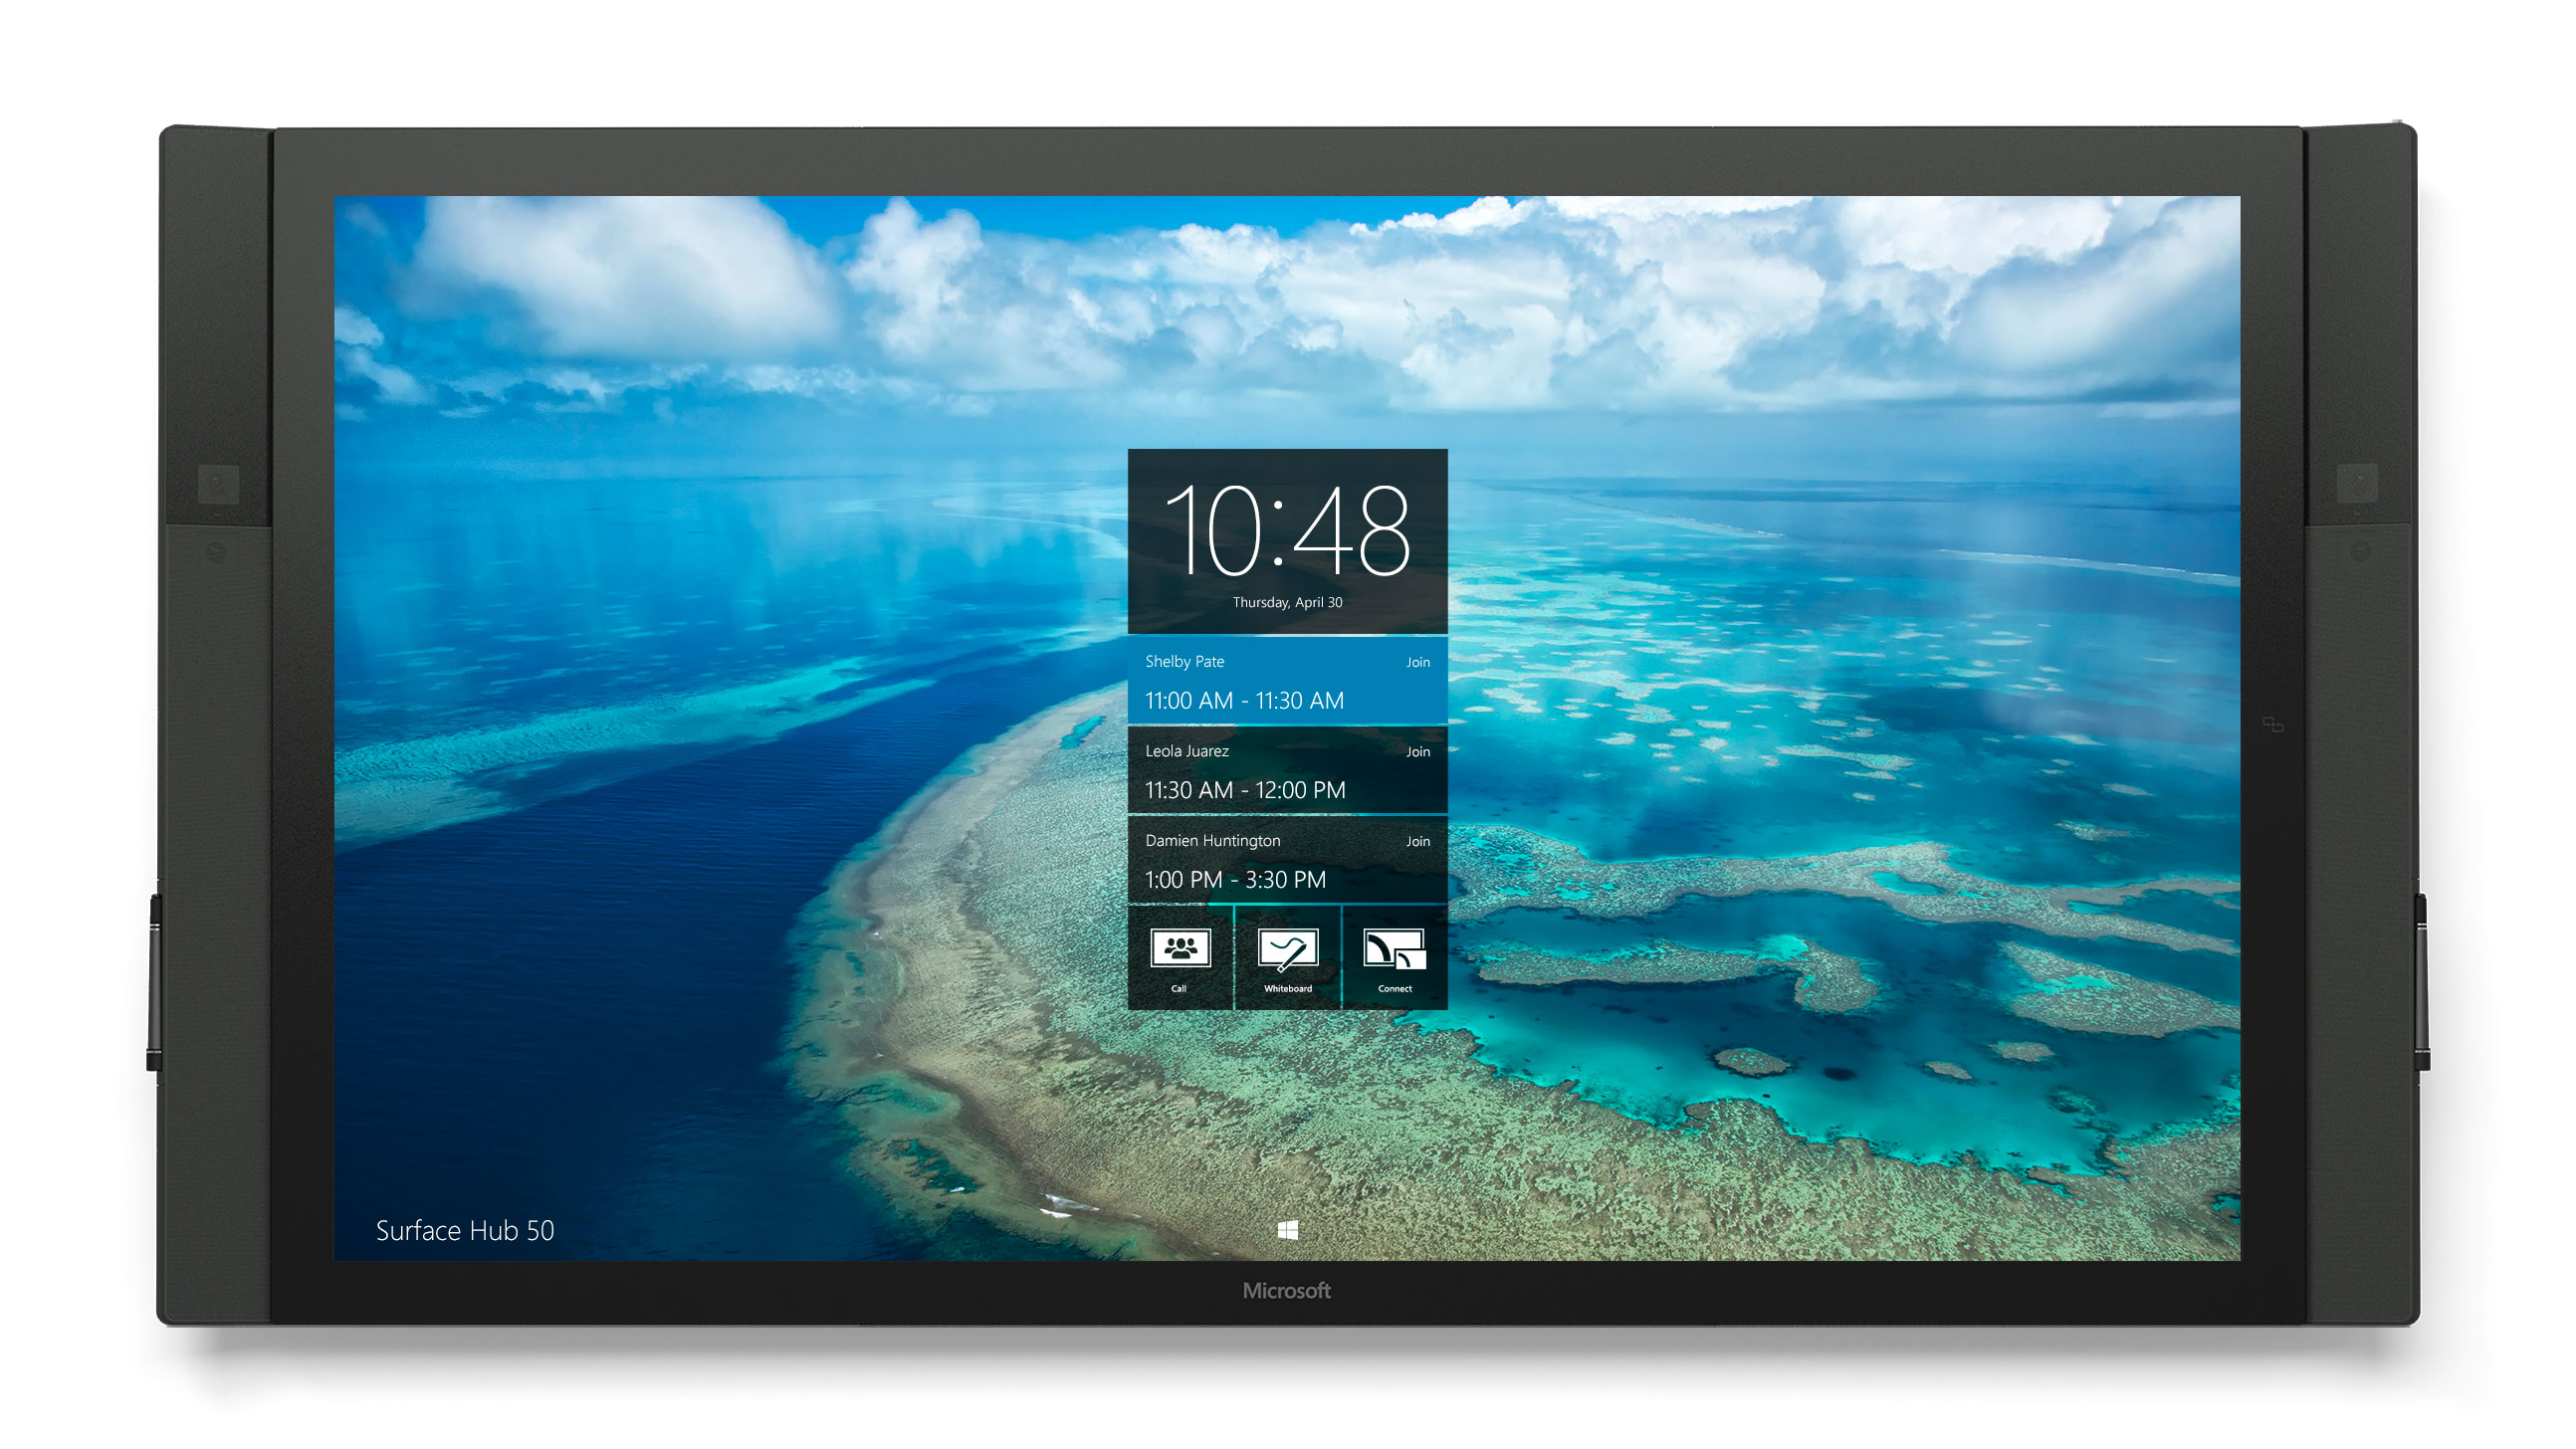
\includegraphics[height=4.5cm,keepaspectratio]{technologies/surface-hub.jpg}
\end{figure}

Surface Hub is a collaborative device from Microsoft. It has a 55-inch touch display with 1920 times 1080 pixel resolution. The main aim of the device is to encourage team work between people and increase their productivity. It has been adapted with various technologies such as wide angle view display, camera and responsive pen. 

The Surface Hub runs Windows 10 Team, which is a customized version of Windows 10 Enterprise operating system. Apart from, as the operating system name itself suggest, using it for collaboration and team work, the Surface Hub operating system creates new session every time when it is started. It doesn't save or store the data and session from previous time. In addition to that, it also doesn't have internal file system.

The Surface Hub has a really good cameras, speakers and microphone. With the software Skype for Business from Microsoft,  which is installed on the device, the Surface Hub can be said as one of the best device for video conferencing. 

